\chapter{%
深層学習による配管6D姿勢推定}

従来のアイソメ図作成方法では3次元点群を取得できるLIDARセンサーを使用することで図面を作成していたが、LIDARセンサーが他のセンサーよりも高価であるというデメリットを抱えているため、一般的に使用することは困難であるとされていた。
そのため、本研究ではLIDARセンサーよりも比較的安価なRGB-Dカメラを用いてデータセット収集からアイソメ図作成までの方法を紹介する。
第2.1節ではRGB-Dカメラを用いた深層学習による配管6D姿勢推定の手順を述べる。
第2.2節では物体認識のネットワーク設計を詳しく説明する。

\section{配管6D姿勢推定方法}
RGB-Dカメラを用いた深層学習による配管のアイソメ図作成の手順はデータ収集、物体検出、6D姿勢推定、アイソメ図作成の4つのステップに分けられる。
図2.1にそのプロセスの流れを示す。

\begin{figure}[htbt]
	\includegraphics[height=65mm]{system.eps}
	\caption{RGB-Dカメラを用いた深層学習によるアイソメ図作成方法}
	\label{fig:f2}
\end{figure}

まず、RGB-Dカメラを用いてRGB画像とDepth画像を取得する。これらの画像を使用して物体検出ネットワークにより複数の配管検出を行う。
次に、物体検出で認識された結果を用いて配管の姿勢をそれぞれのオブジェクトごとに推定する。その際に使用するデータセットは3次元復元ツールであるColmapを使用して生成された配管の点群データである。
姿勢推定を行った後、アイソメ図に配管のスケール情報を示す必要があるため、Depth画像を用いて認識された配管同士の距離を算出する。
以上で出力された結果を用いて姿勢推定された値と配管のスケール情報を使用しアイソメ図を作成する。\\
しかし、本研究では配管の物体検出、姿勢推定、スケール算出までの工程は成し遂げたが、時間の都合上、アイソメ図を作成することができなかったためそれまでの工程の検証結果を紹介する。

\section{配管の特徴を活かしたアイソメ図作成方法}
アイソメ図作成には配管の特徴を活かした効率的な手法を提案する。図2.2に一部配管の例を示す。
一般的な配管は両端部分の曲管やT字管などのつなぎ目を除くと直管であるという特徴がある。そのため、両端の曲管がどの方向を向いているのかを推論できれば向かい合っている曲管のペアを見つけられ、その間を直線で結ぶことで
アイソメ図を描画することができる。そのため、本研究においては配管全体を認識するのではなく、配管のつなぎ目である曲管及びT字管を物体検出と姿勢推定を用いて推論する。

\begin{figure}[htbt]
	\centering
	 \includegraphics[height=55mm]{pipe.eps}
	 \caption{配管の検出例}
	 \label{fig:f2}
\end{figure}


\section{ネットワーク構造}
\subsection{RXDネットワーク}

本研究の物体検出に使用するネットワークにRXDモデルを提案する。RXDネットワークの構成を図2.4に示す。認識ネットワークに入力するRGB画像とDepth画像はそれぞれ416x416のサイズに縮小する。
このサイズに固定する理由は、解像度を落とすことで計算量を減らすとともに、縮小による画像情報の損失がないようにするためである。縮小された画像はそれぞれConvolutional setに
通して、複数の畳み込み層によって入力画像を解像度を下げるとともに、画像から特徴マップを抽出することができる。Convolutional setにはBatch Normalization(BN)、ReLU、Max Pooling(MP)を各層に取り入れている。
Batch Normalizationは各バッチのデータを使用し正規化を行う。その結果、出力が適度に分散され、勾配消失などの問題が起こりにくくなり学習が適切に進む。特にネットワークの層が深いモデルを使用した際に、Batch Normalizationを挿入することで効果を発揮する。
次に、活性化関数であるReLU層について紹介する。活性化関数にはReLU関数やSigmoid関数などが有名であり、それぞれのグラフを図2.3, 図2.4に示す。ReLUは関数への入力値が0以下の場合に出力値が常に0、入力値が0より上の場合には出力値が同じ値を示す関数である。ReLU関数の特徴は勾配消失の問題を改善できるメリットがある。
最後にMax PoolingはCNNで用いられる基本的なプーリング層である。Map Poolingでは各位置のカーネル内の最大値のみを残すプーリング処理である。プーリング層では畳み込みによって得られた特徴マップが平行移動などが起きても影響を及ぼさないようにロバスト性を与えることができる。
これらの層を複数回使用することで層を重ねるごとに解像度を下げるとともに特徴をより濃いものとして出力される。Convolutionl setを複数回通すと、次はRXD層を使用することになる。RXD層の詳細に関しては2.3.2で紹介する。
RXD層を通過すると最後はPredict層によってっ曲管とT字管の推定結果を得ることができる。このPredict層はYOLOで使用されているYOLO Layerを使用している.RXDネットワークはPredict層が3つ存在しているが、これは様々なスケールの物体に対応するために、
特徴マップの大きさに応じて3つの出力層があり、それぞれのPredict層で出力または損失をを求める。

\begin{figure}[htbp]
  \begin{minipage}[b]{0.45\linewidth}
    \centering
    \includegraphics[keepaspectratio, scale=0.35]{relu.eps}
    \caption{ReLU関数}
  \end{minipage}
  \begin{minipage}[b]{0.45\linewidth}
    \centering
    \includegraphics[keepaspectratio, scale=0.35]{sigmoid.eps}
    \caption{Sigmoid関数}
  \end{minipage}
\end{figure}

\clearpage

\begin{figure}[htbt]
	\centering
	 \includegraphics[height=95mm]{rxdnet.eps}
	 \caption{RXDネットワーク構造図}
	 \label{fig:f2}
\end{figure}

\begin{figure}[htbt]
	\centering
	 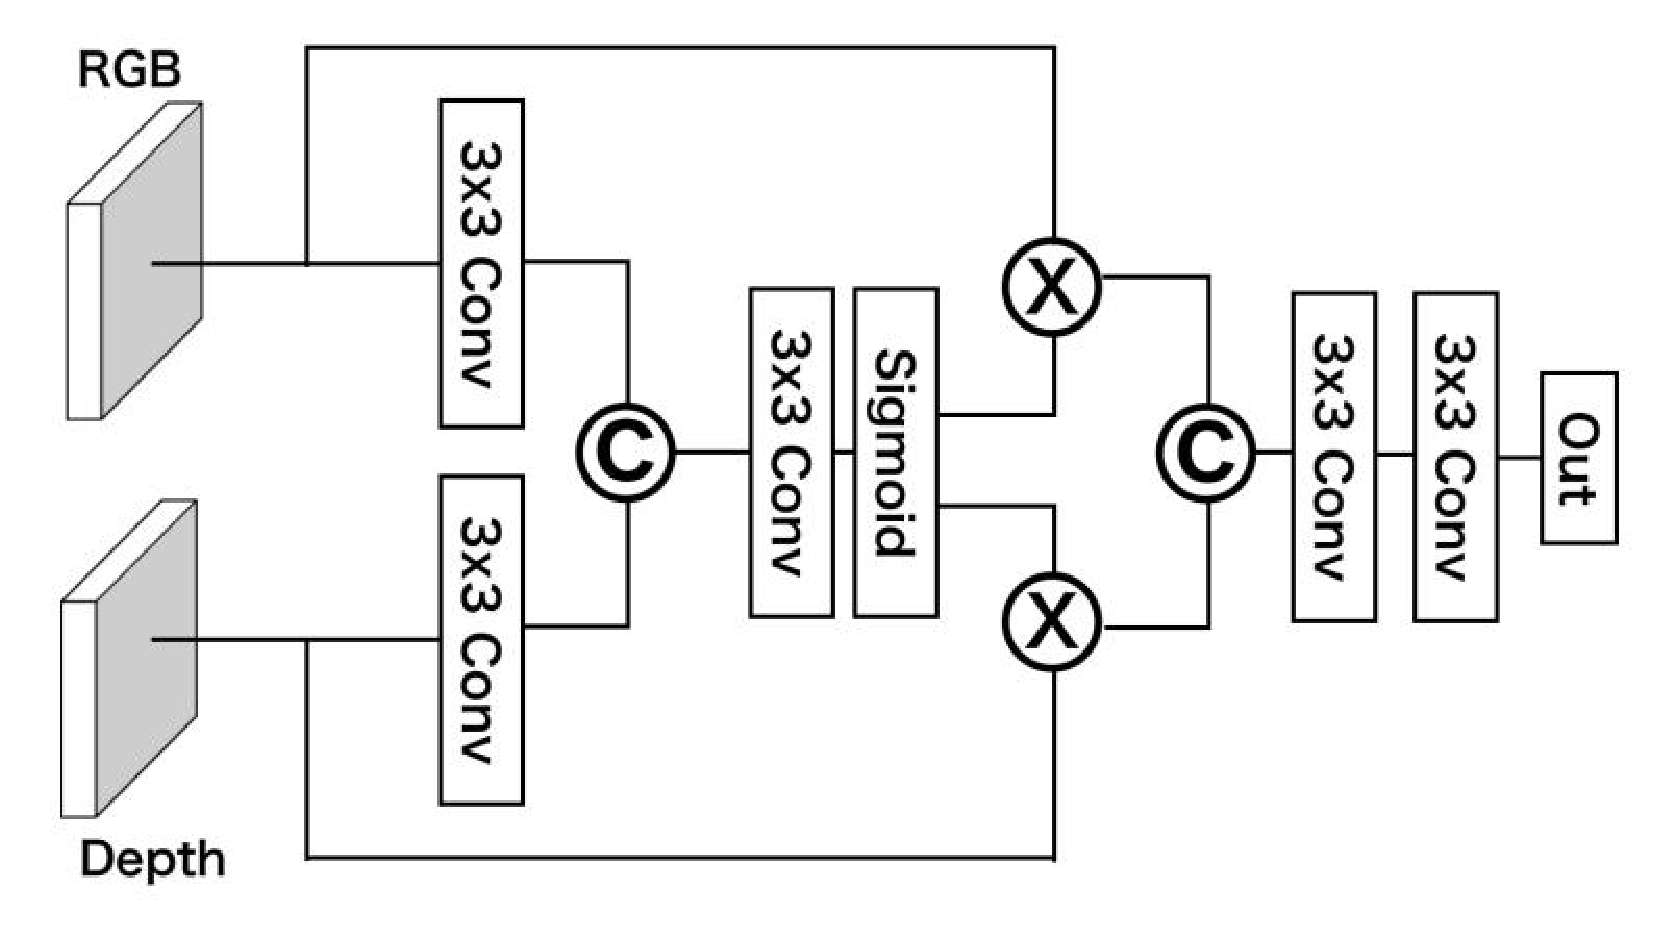
\includegraphics[height=85mm]{RXD.eps}
	 \caption{RXD層}
	 \label{fig:f2}
\end{figure}

\subsection{RXD層}
RXD層の内部構成を図2.5に示す。RXD層の中身ではRGB画像とDepth画像がRXDネットワークで畳み込まれたデータを結合する役割を担っている。
まず、入力画像であるRGB画像とDepth画像をそれぞれ1x1の畳み込み層を使用してチャネル数を半減させる。チャネル数を減少させることで使用されるパラメータ数を抑制し学習の高速化を狙う目的がある。
それらのデータをConcatenate関数を用いてそれぞれのテンソルを結合する次元を指定することでRGB画像とDepth画像の配列を一つの変数に置き換えることができる。
ここでRGB画像とDepth画像の特徴マップを連結することに成功するが、テンソルを繋げ合わしたのみで、まだそれぞれの特性の相関関係を共有することはできていない。
次に、結合されたデータを3x3の畳み込み層を使用し、特徴を抽出したあとはSigmoid関数という活性化関数を使用する。RXDネットワークのConvolution setでは活性化関数にReLU関数が使用され、
入力が0以下の時は0を、0より大きい時はその値を出力していた。しかし、Sigmoid関数はReLU関数とは違い、入力値xの値に依らず0~1の数値に変換して出力する。
次のステップではRXDネットワークから入力された元のデータとSigmoid関数によって出力されたマップを乗算する。このステップによりRGB画像とDepth画像の
それぞれの特性を維持したまま相関を共有することができる。これによって得られたそれぞれの値をConcatenate関数を用いることで再度結合し、
2度の畳み込み層を経ることで完結する。



